\chapter{Results and Discussion}
\section{Stability Analysis in 10 Bus 4 Generator System}
\label{contingency1}
A realistic 4-machine 10-bust network design is presented to demonstrate the working of the suggested Catastrophic indicator. The organization's graphical chart can be found in Fig. \ref{fig:Line Diagram}. Prepare a model dataset as follows:
\begin{enumerate}
\item A consistent state working point is designated a base powerflow.
\item At 0.5 s, a three-stage cutoff is implemented at bus 9. (Tfault).
\item By opening the line between bus 9 and bus 10, the deficiency is resolved in 0.1 second (Tclear) (line possibility).

\end{enumerate}

\begin{figure}[H]
  \centering
  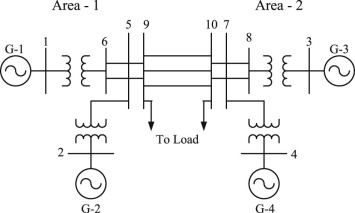
\includegraphics[width=0.6\linewidth]{LD}
  \caption{Line Diagram of two area 4 Machine 10 Bus Power System}
  \label{fig:Line Diagram}
\end{figure}

Initially the assumed fault is provided to the each bus system and the system parameters are observed. The further steps as described in Algorithm \ref{Computation of Indicators} are carried out using set of codes. So, assuming the fault initiated at 0.5 sec, for different fault clearing time, the faulted bus is provided for observing the transient stability result.

\subsection{Results for Indicator based on Coherency}
\label{Ind1}
\begin{figure}[H]
\centering
\begin{subfigure}{.5\textwidth}
  \centering
  \includegraphics[width=\linewidth]{Co No fault}
  \caption{Speed Deviation Vs. Time for No Fault}
  \label{fig:I1sub1}
\end{subfigure}%
\begin{subfigure}{.5\textwidth}
  \centering
  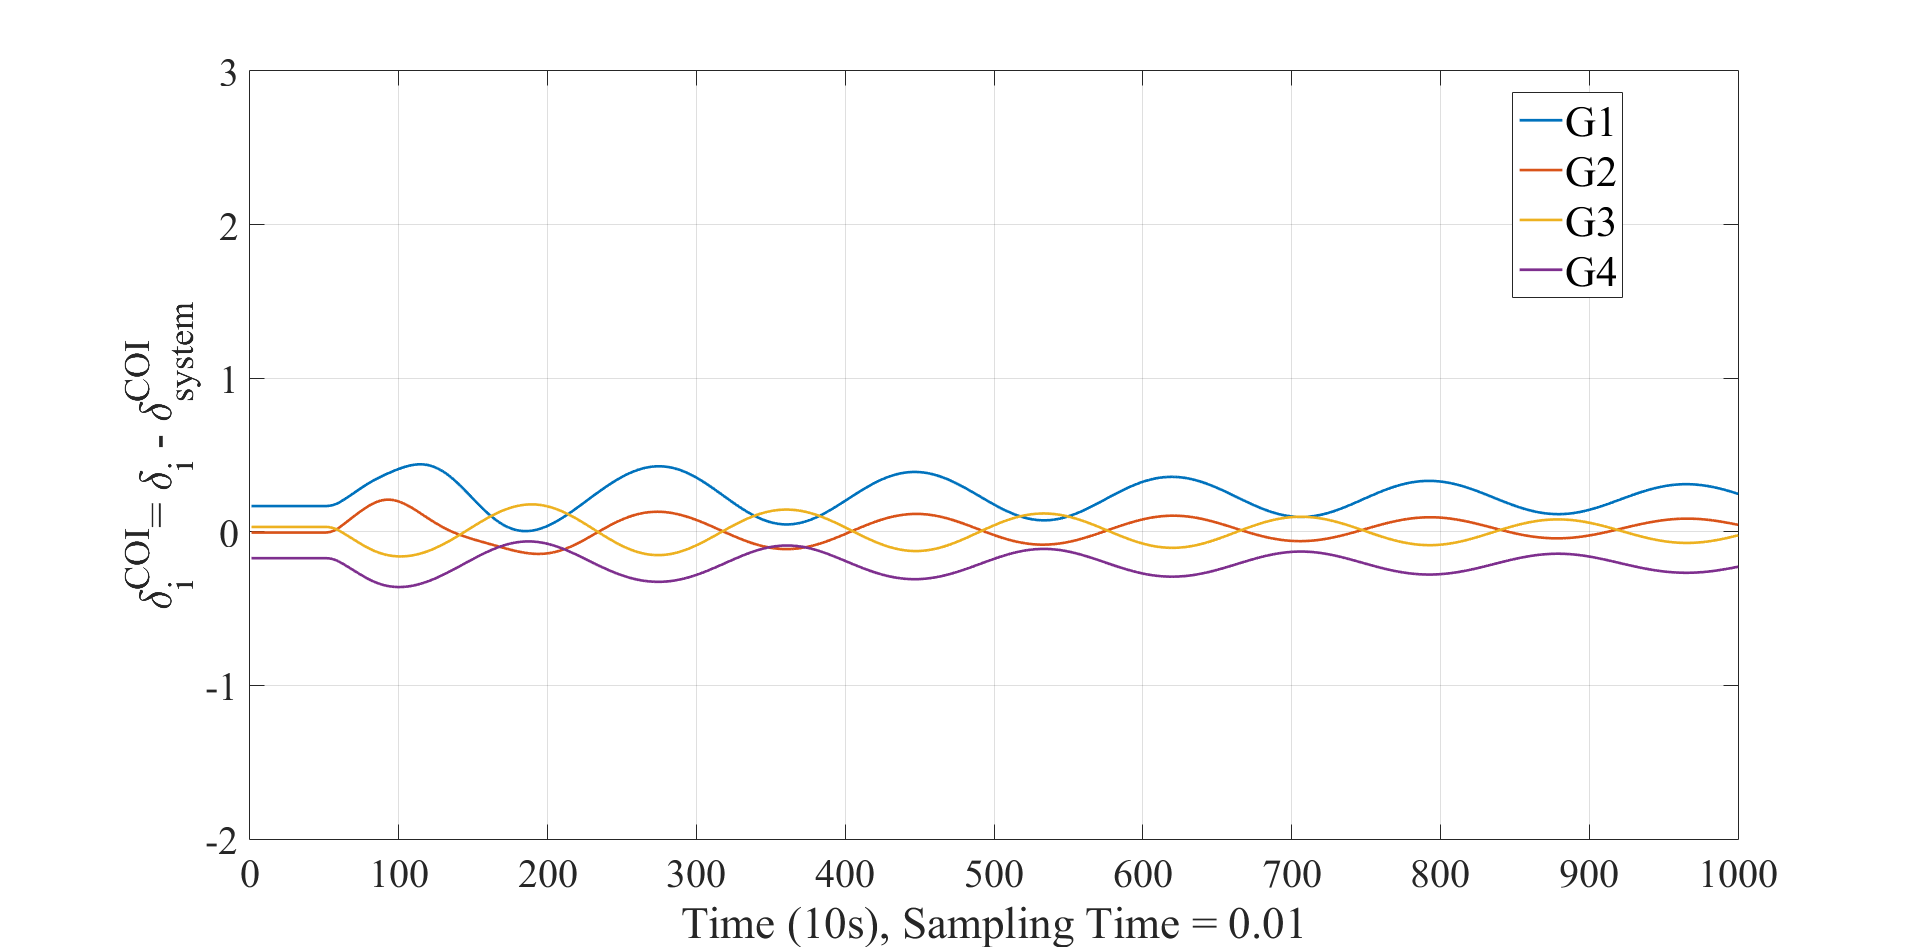
\includegraphics[width=\linewidth]{Co A1}
  \caption{Speed Deviation Vs. Time for \(T_c\) = 0.1 sec}
  \label{fig:I1sub2}
\end{subfigure}
\\
\begin{subfigure}{.5\textwidth}
  \centering
  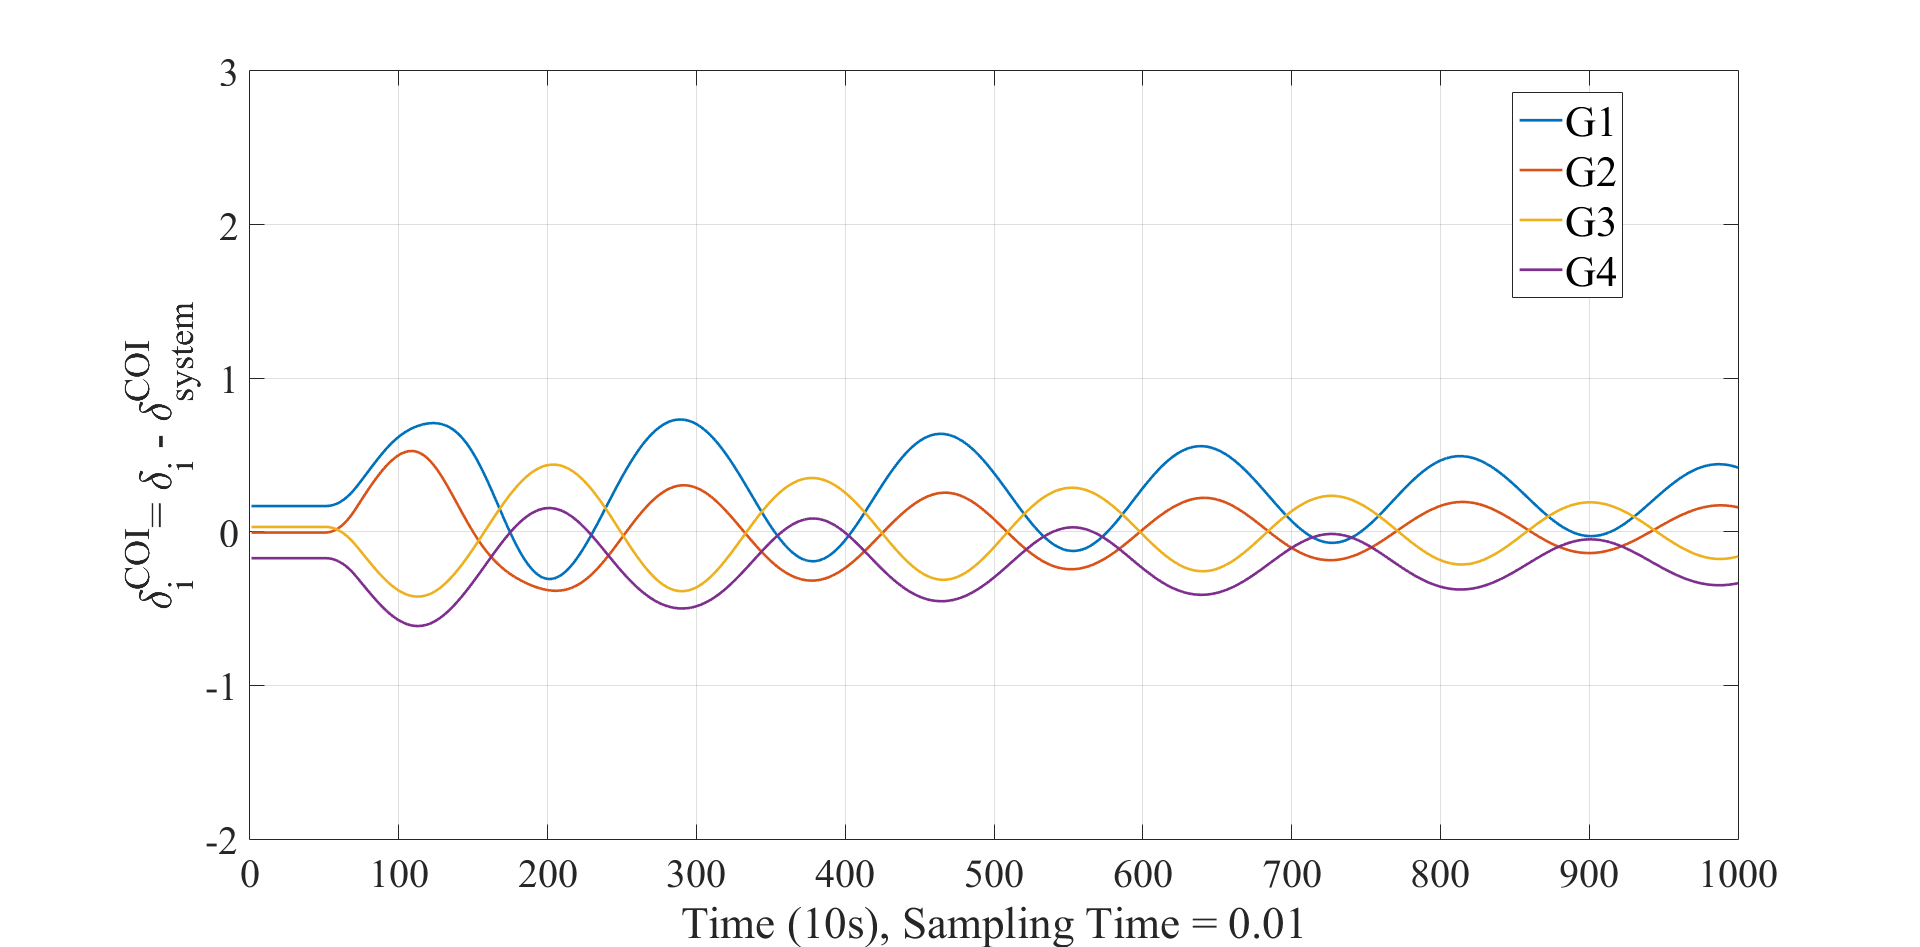
\includegraphics[width=\linewidth]{Co A2}
  \caption{Speed Deviation Vs. Time for \(T_c\) = 0.2 sec}
  \label{fig:I1sub3}
\end{subfigure}%
\begin{subfigure}{.5\textwidth}
  \centering
  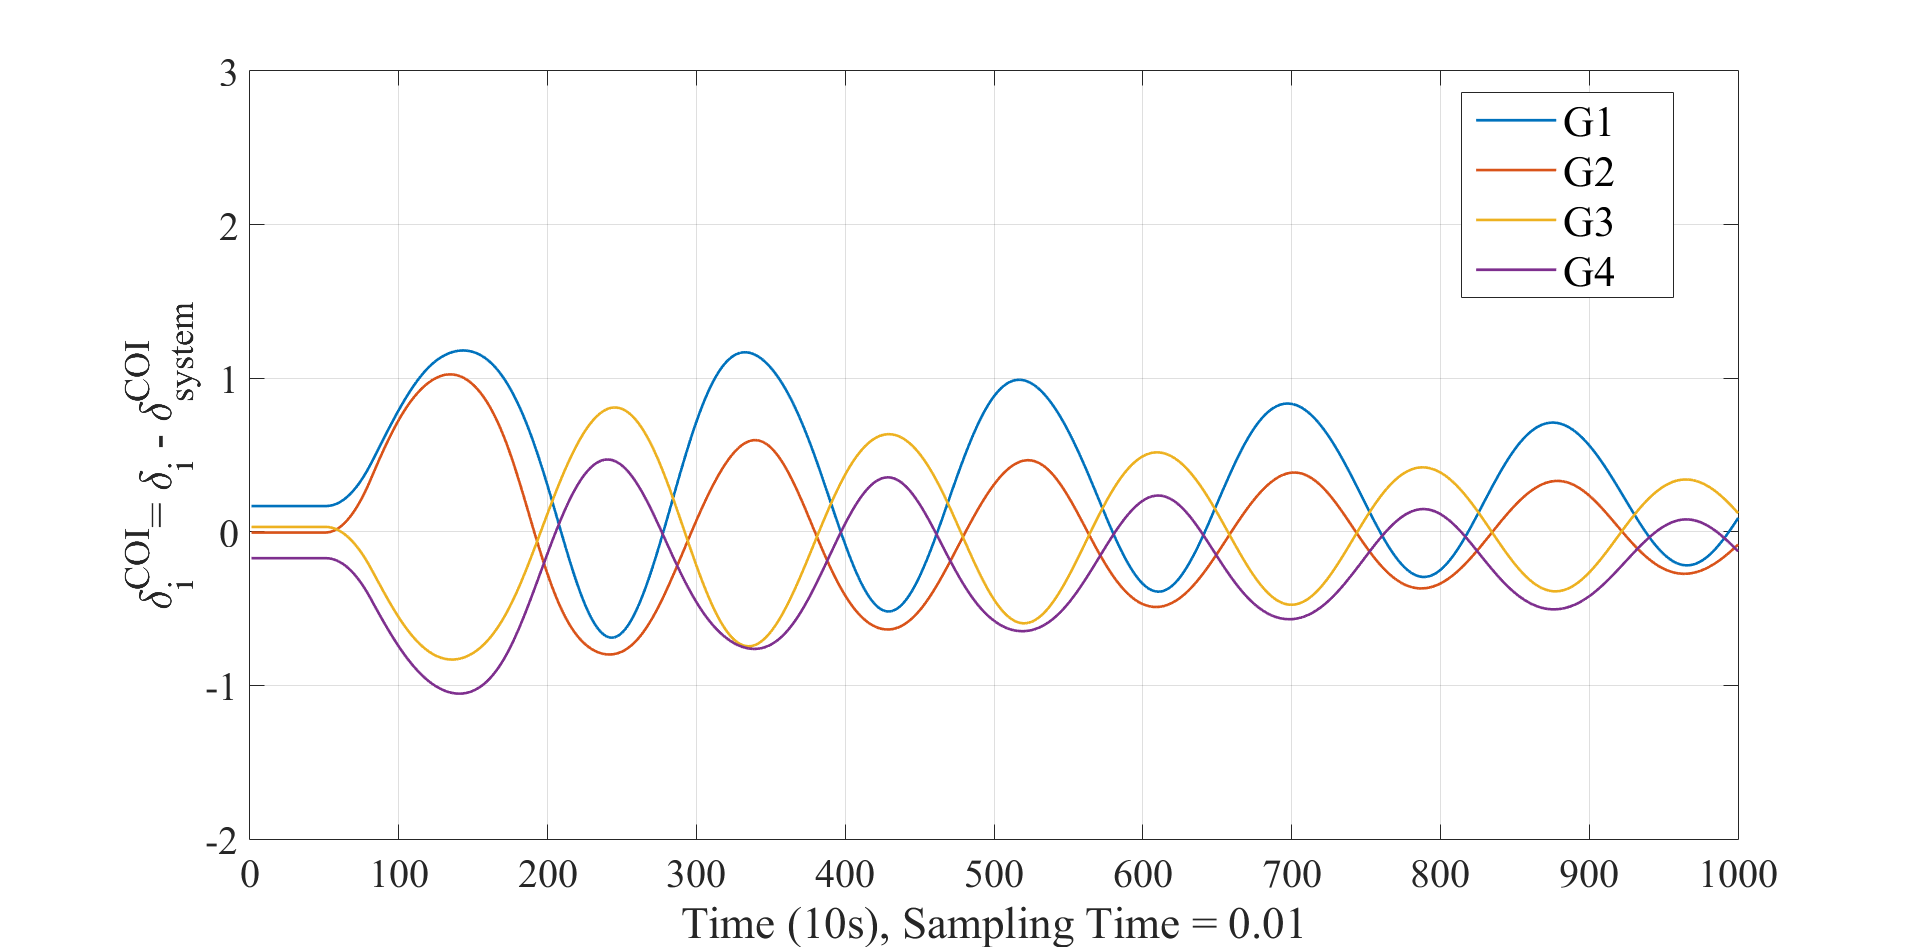
\includegraphics[width=\linewidth]{Co A3}
  \caption{Speed Deviation Vs. Time for \(T_c\) = 0.3 sec}
  \label{fig:I1sub4}
\end{subfigure}
\\
\begin{subfigure}{.5\textwidth}
  \centering
  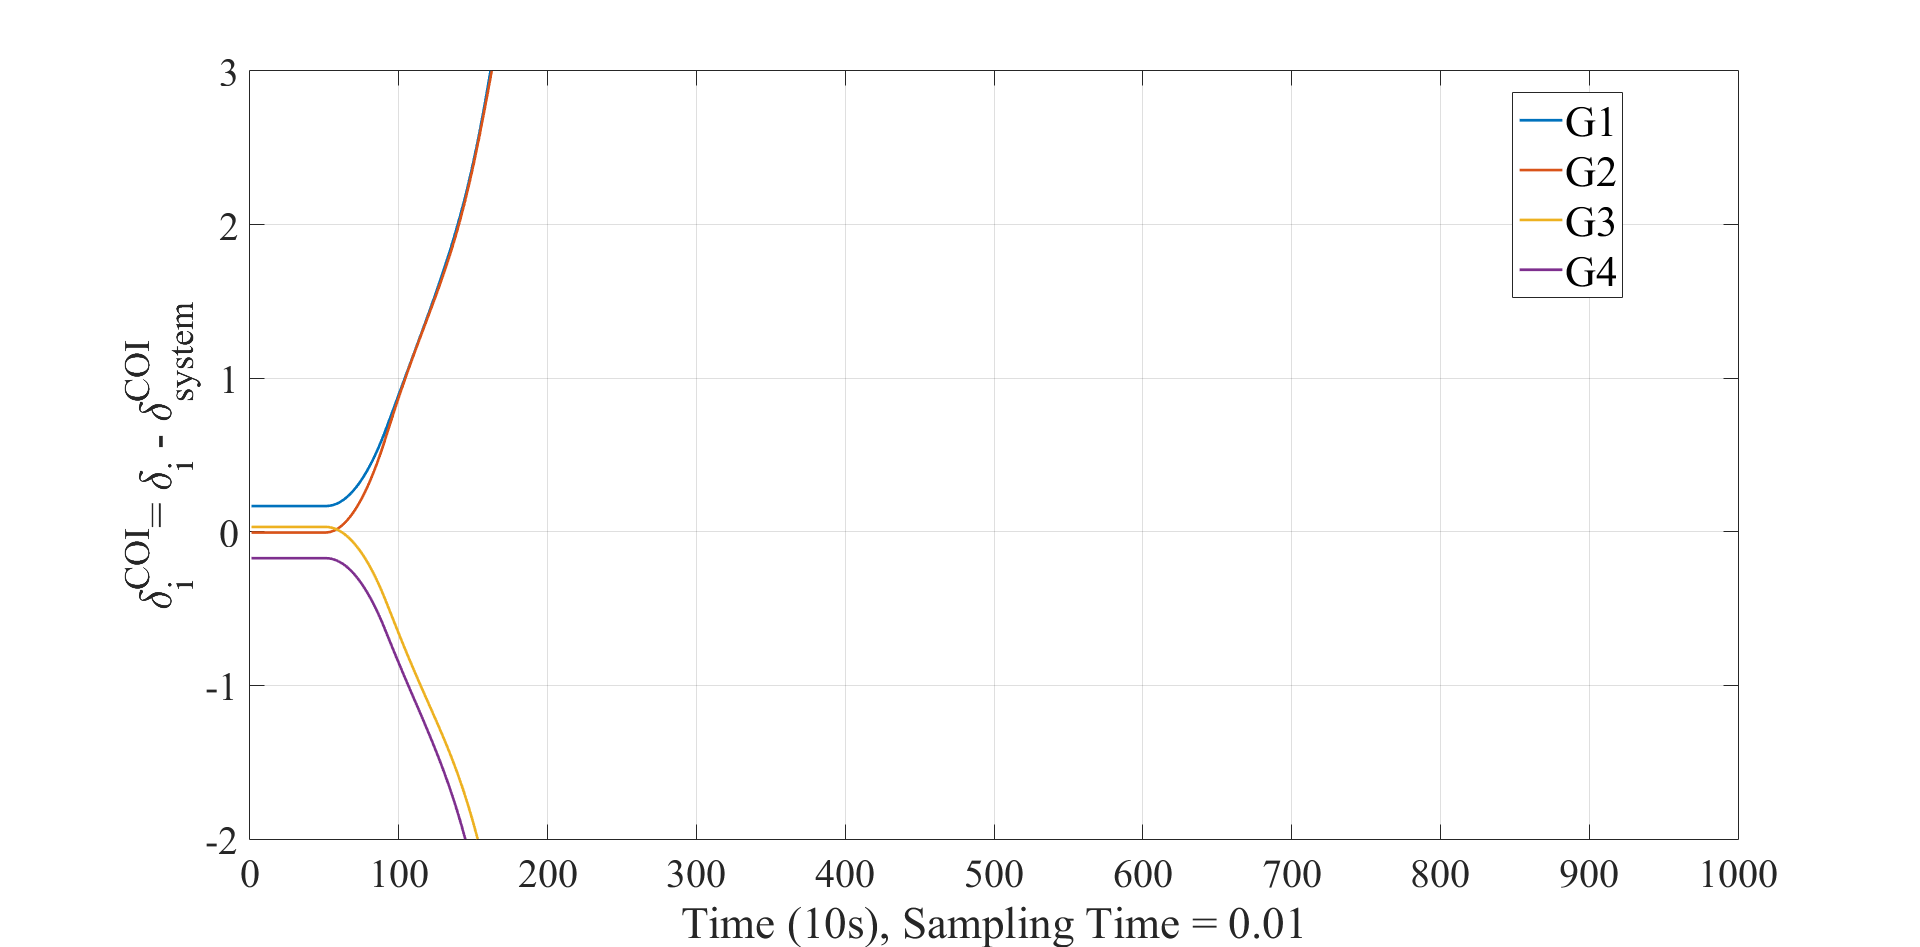
\includegraphics[width=\linewidth]{Co A4}
  \caption{Speed Deviation Vs. Time for \(T_c\) = 0.4 sec}
  \label{fig:I1sub5}
\end{subfigure}
\caption{Indicator based on Coherency}
\label{fig:I1}
\end{figure}

\begin{table}[H]
\renewcommand{\arraystretch}{1}
\caption{Contingency Analysis using Indicator based on Coherency}
\label{Table:I1}
\begin{center}
\begin{tabular}{|P{0.3\linewidth} | P{0.3\linewidth} | P{0.2\linewidth}|}
\hline
 \textbf{Fault Clearing Time} & \textbf{Performance Index} & \textbf{Remarks}  \\ \hline
 No Fault & 1.7262e-10  & Stable \\ \hline
 0.1 sec & 0.4349  & Stable \\ \hline
 0.2 sec & 1.0385  & Stable \\ \hline
 0.3 sec & 1.8697  & Stable \\ \hline
 0.4 sec & 66.9471  & Unstable \\ \hline
 
\end{tabular}
\end{center}
\end{table}




\subsection{Results for Indicator based on Transient Energy Conversion}
\label{Ind2}
\begin{figure}[H]
\centering
\begin{subfigure}{.5\textwidth}
  \centering
  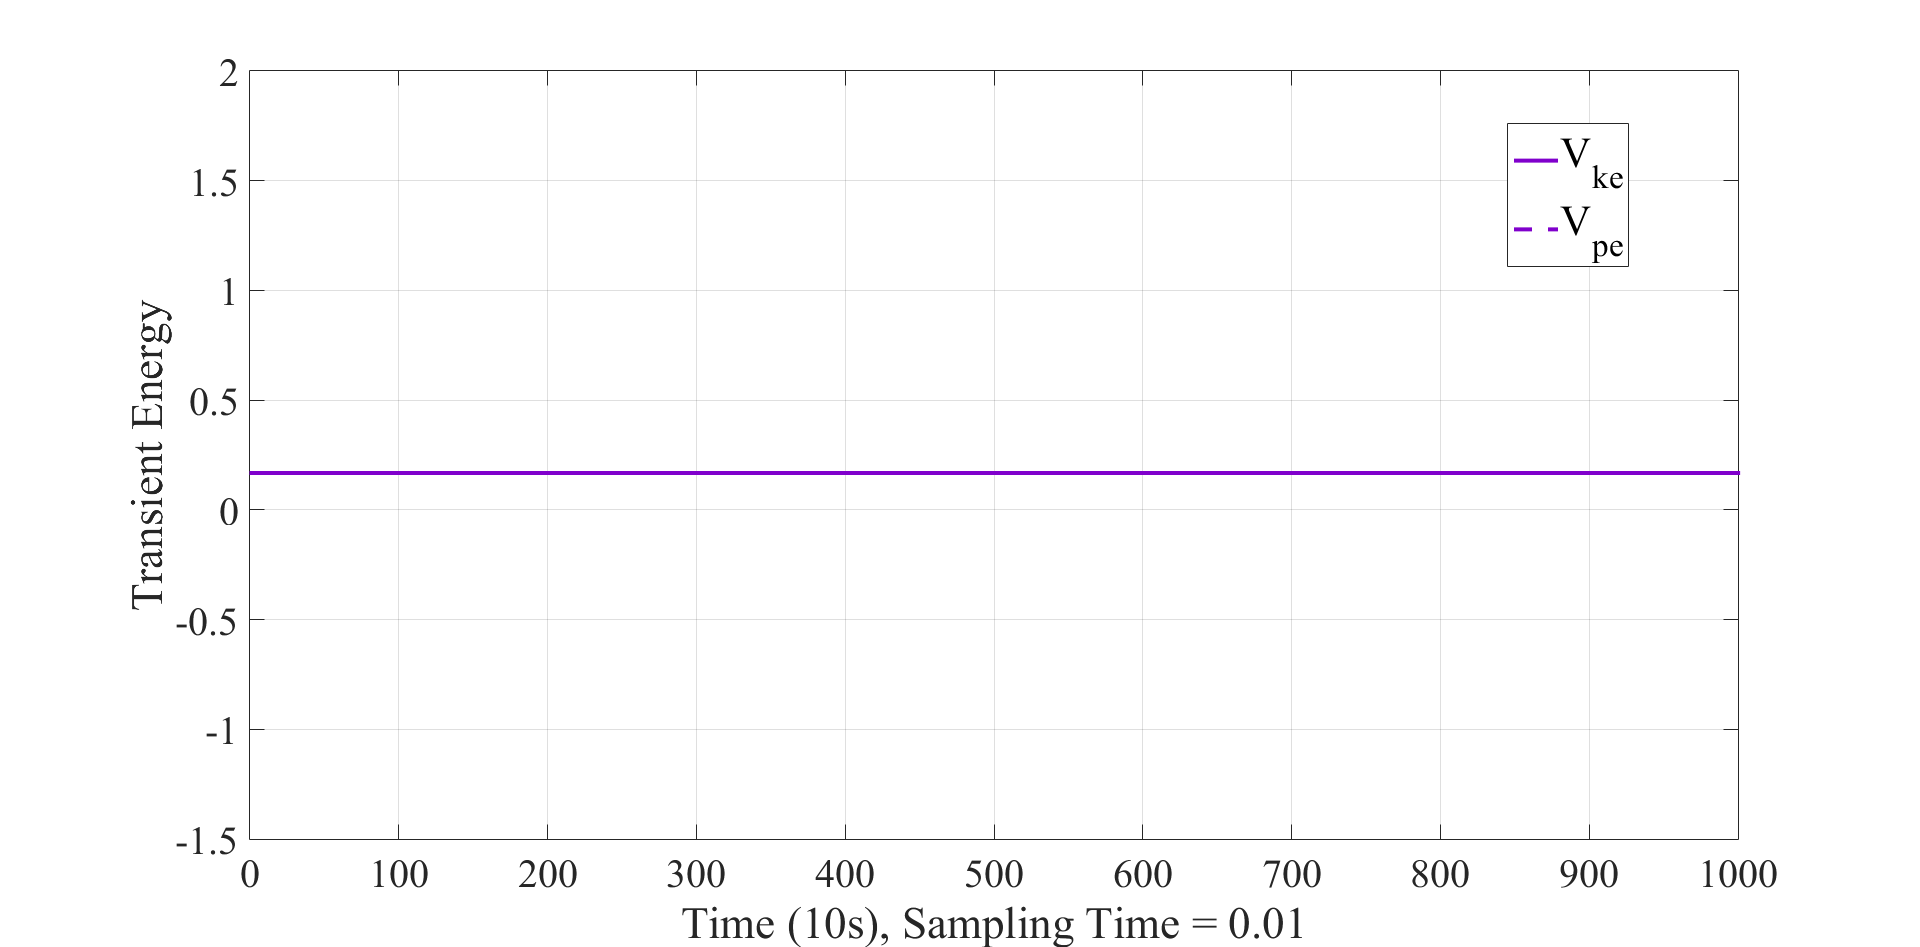
\includegraphics[width=\linewidth]{TE No Fault}
  \caption{Transient Energy Vs. Time for No Fault}
  \label{fig:I2sub1}
\end{subfigure}%
\begin{subfigure}{.5\textwidth}
  \centering
  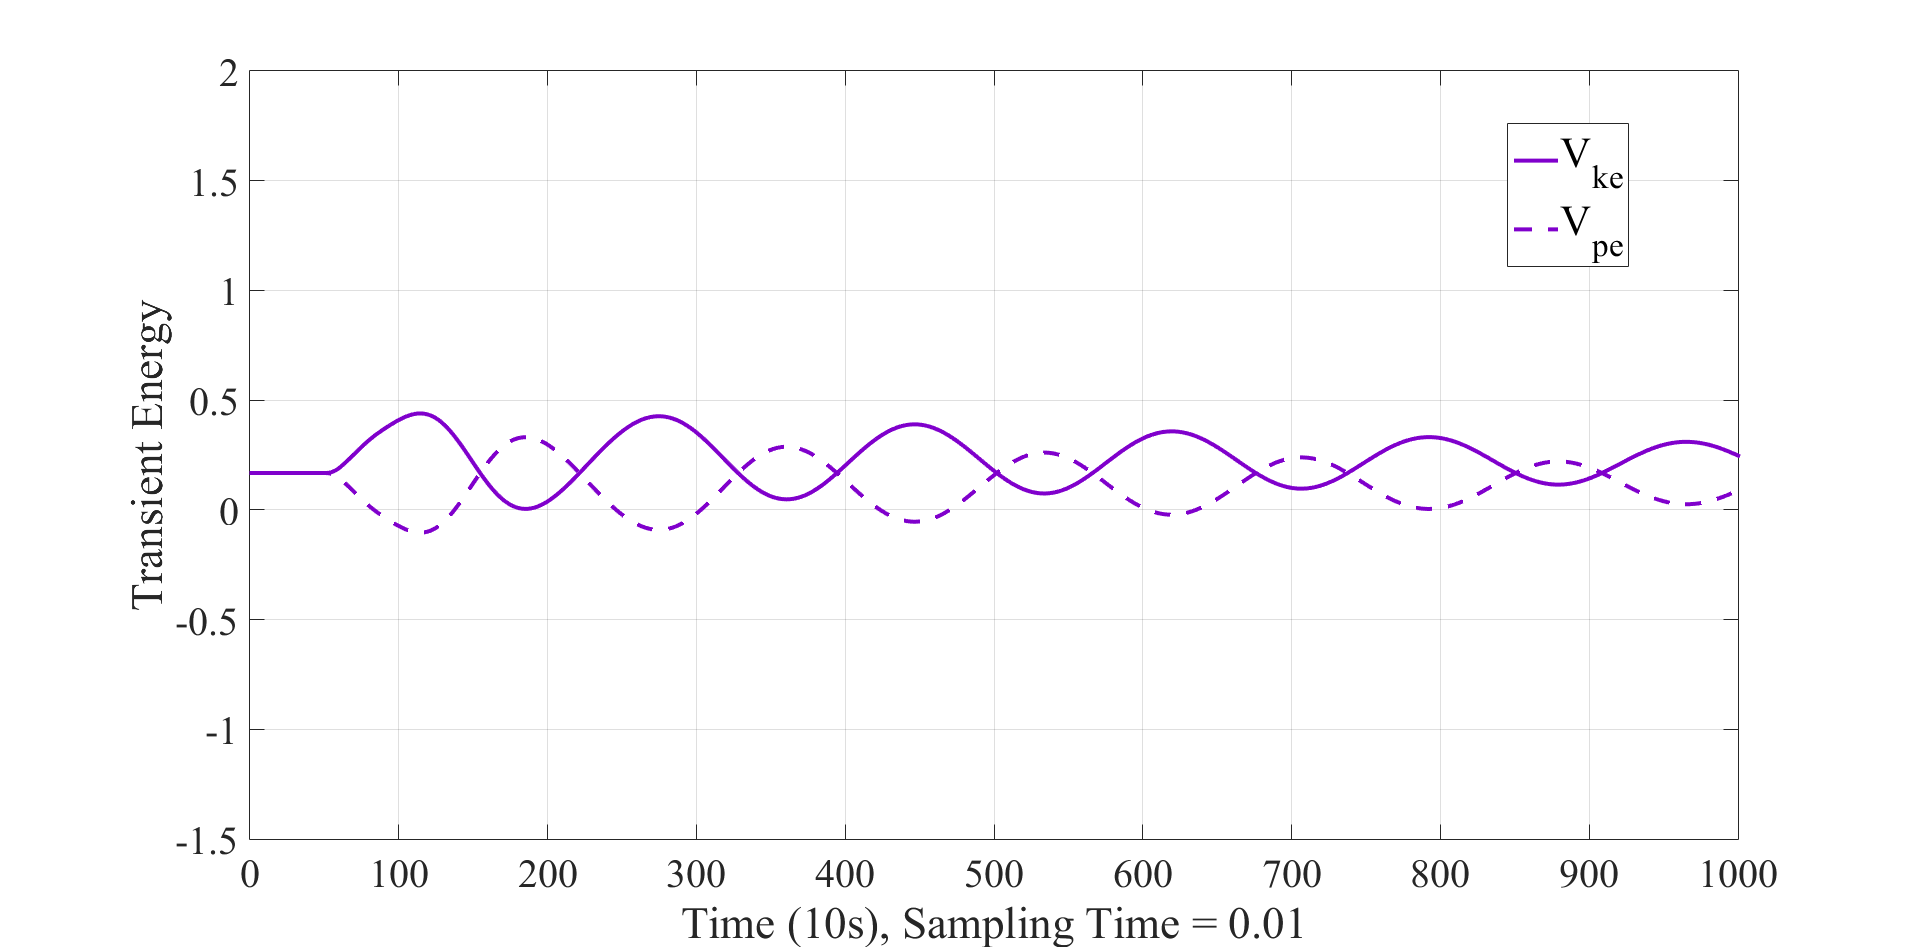
\includegraphics[width=\linewidth]{TE A1}
  \caption{Transient Energy Vs. Time for \(T_c\) = 0.1 sec}
  \label{fig:I2sub2}
\end{subfigure}
\\
\begin{subfigure}{.5\textwidth}
  \centering
  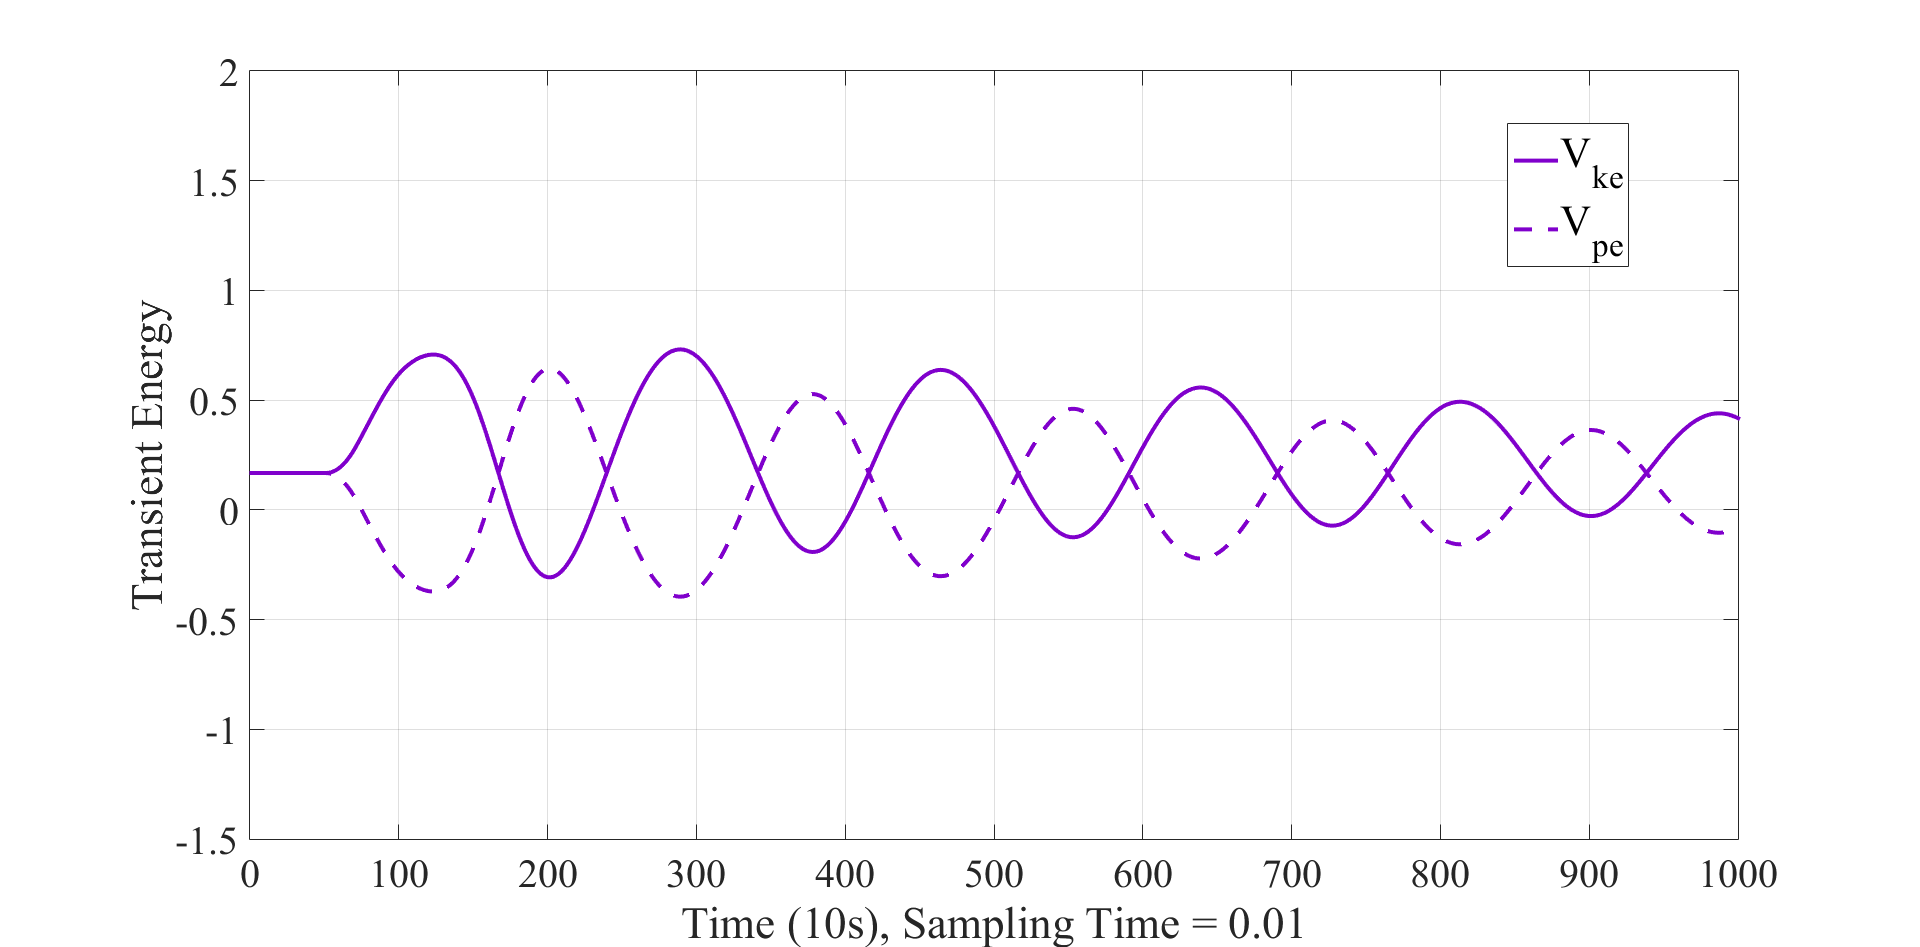
\includegraphics[width=\linewidth]{TE A2}
  \caption{Transient Energy Vs. Time for \(T_c\) = 0.2 sec}
  \label{fig:I2sub3}
\end{subfigure}%
\begin{subfigure}{.5\textwidth}
  \centering
  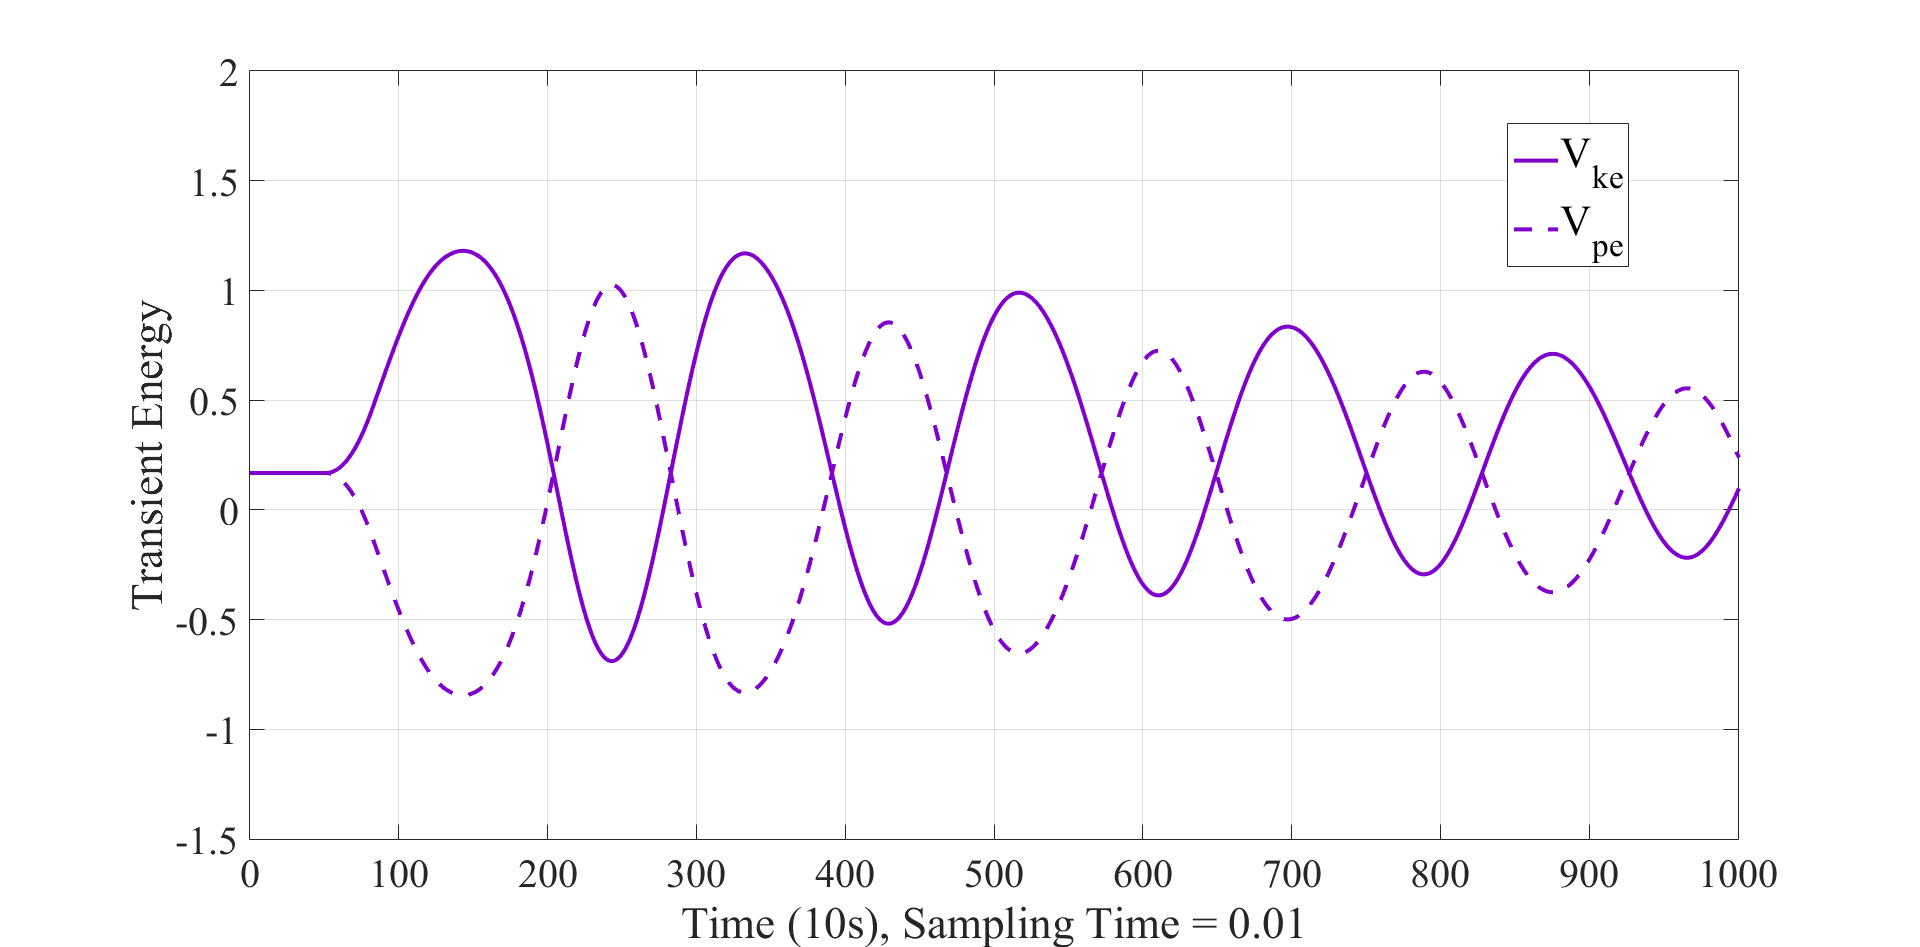
\includegraphics[width=\linewidth]{TE A3}
  \caption{Transient Energy Vs. Time for \(T_c\) = 0.3 sec}
  \label{fig:I2sub4}
\end{subfigure}
\\
\begin{subfigure}{.5\textwidth}
  \centering
  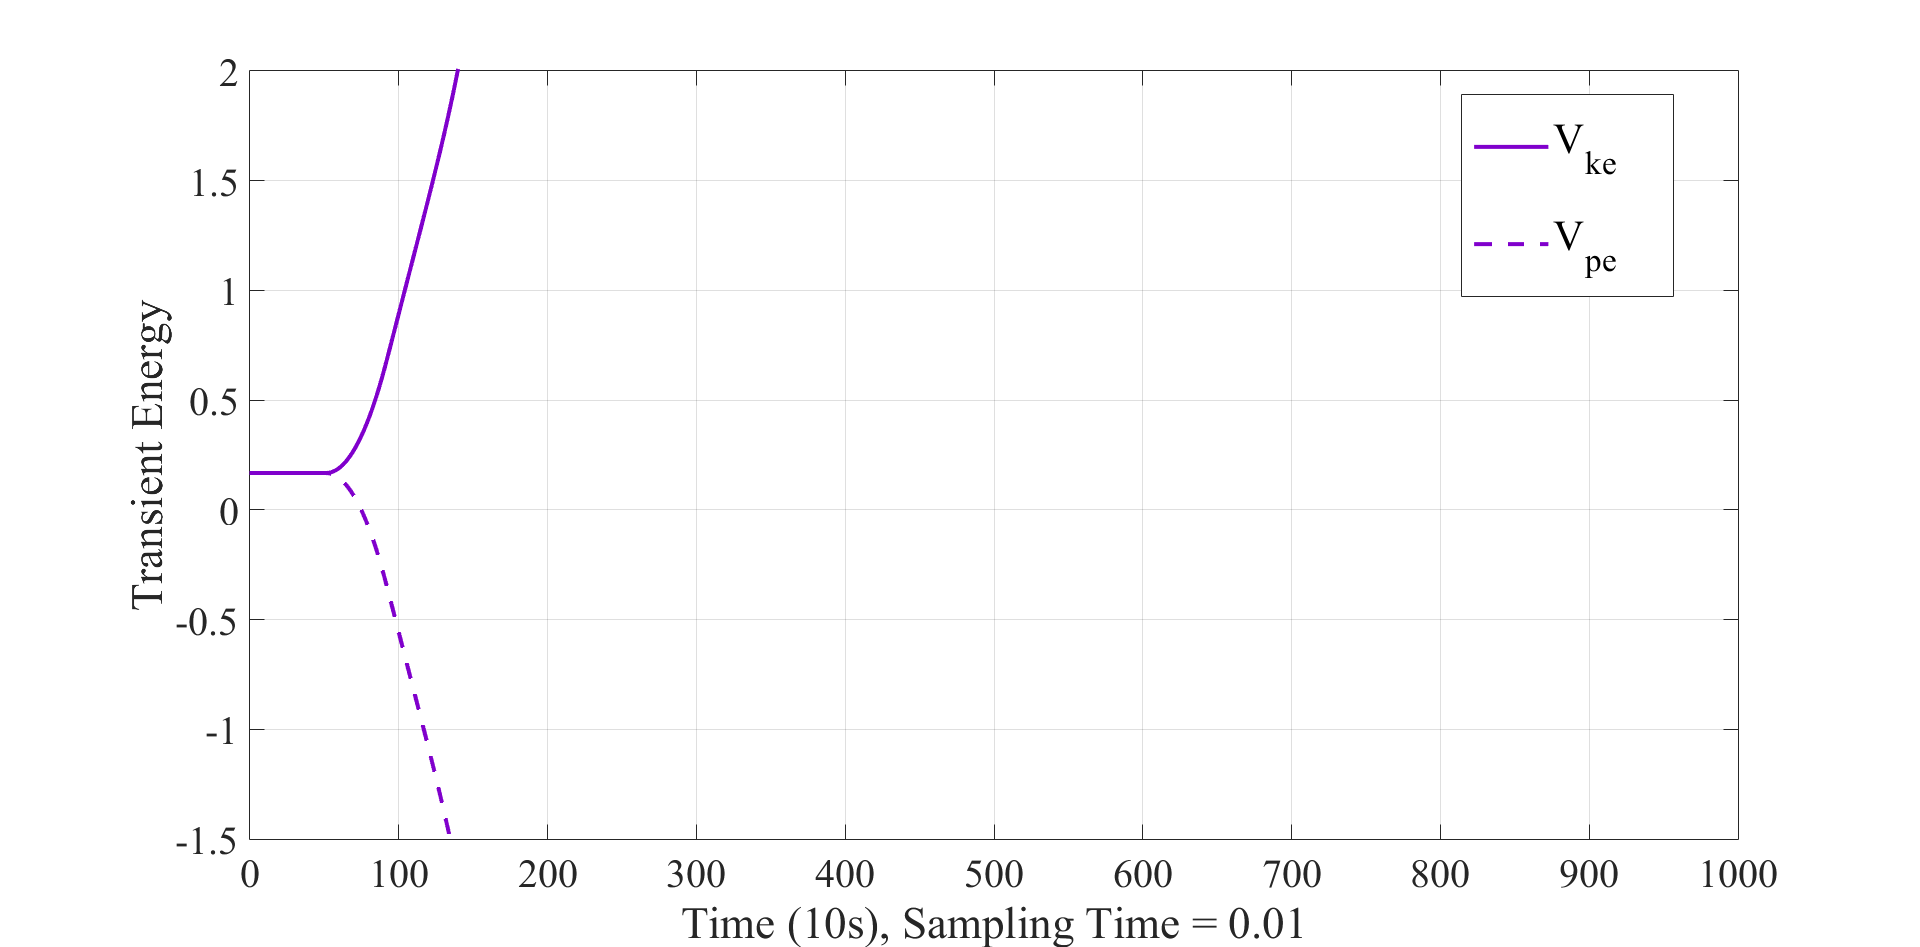
\includegraphics[width=\linewidth]{TE A4}
  \caption{Transient Energy Vs. Time for \(T_c\) = 0.4 sec}
  \label{fig:I2sub5}
\end{subfigure}
\caption{Indicator based on Transient Energy Conversion}
\label{fig:I2}
\end{figure}

\begin{table}[H]
\renewcommand{\arraystretch}{1}
\caption{Contingency Analysis using Indicator based on Transient Energy Conversion}
\label{Table:I2}
\begin{center}
\begin{tabular}{|P{0.3\linewidth} | P{0.3\linewidth} | P{0.2\linewidth}|}
\hline
 \textbf{Fault Clearing Time} & \textbf{Performance Index} & \textbf{Remarks}  \\ \hline
 No Fault & 3.3922e-10  & Stable \\ \hline
 0.1 sec & 0.5432  & Stable \\ \hline
 0.2 sec & 1.1266  & Stable \\ \hline
 0.3 sec & 2.0253  & Stable \\ \hline
 0.4 sec & 133.8941  & Unstable \\ \hline
 
\end{tabular}
\end{center}
\end{table}



\subsection{Results for Indicator based on Dot Products (CSA)}
\label{Ind3}
\begin{figure}[H]
  \centering
  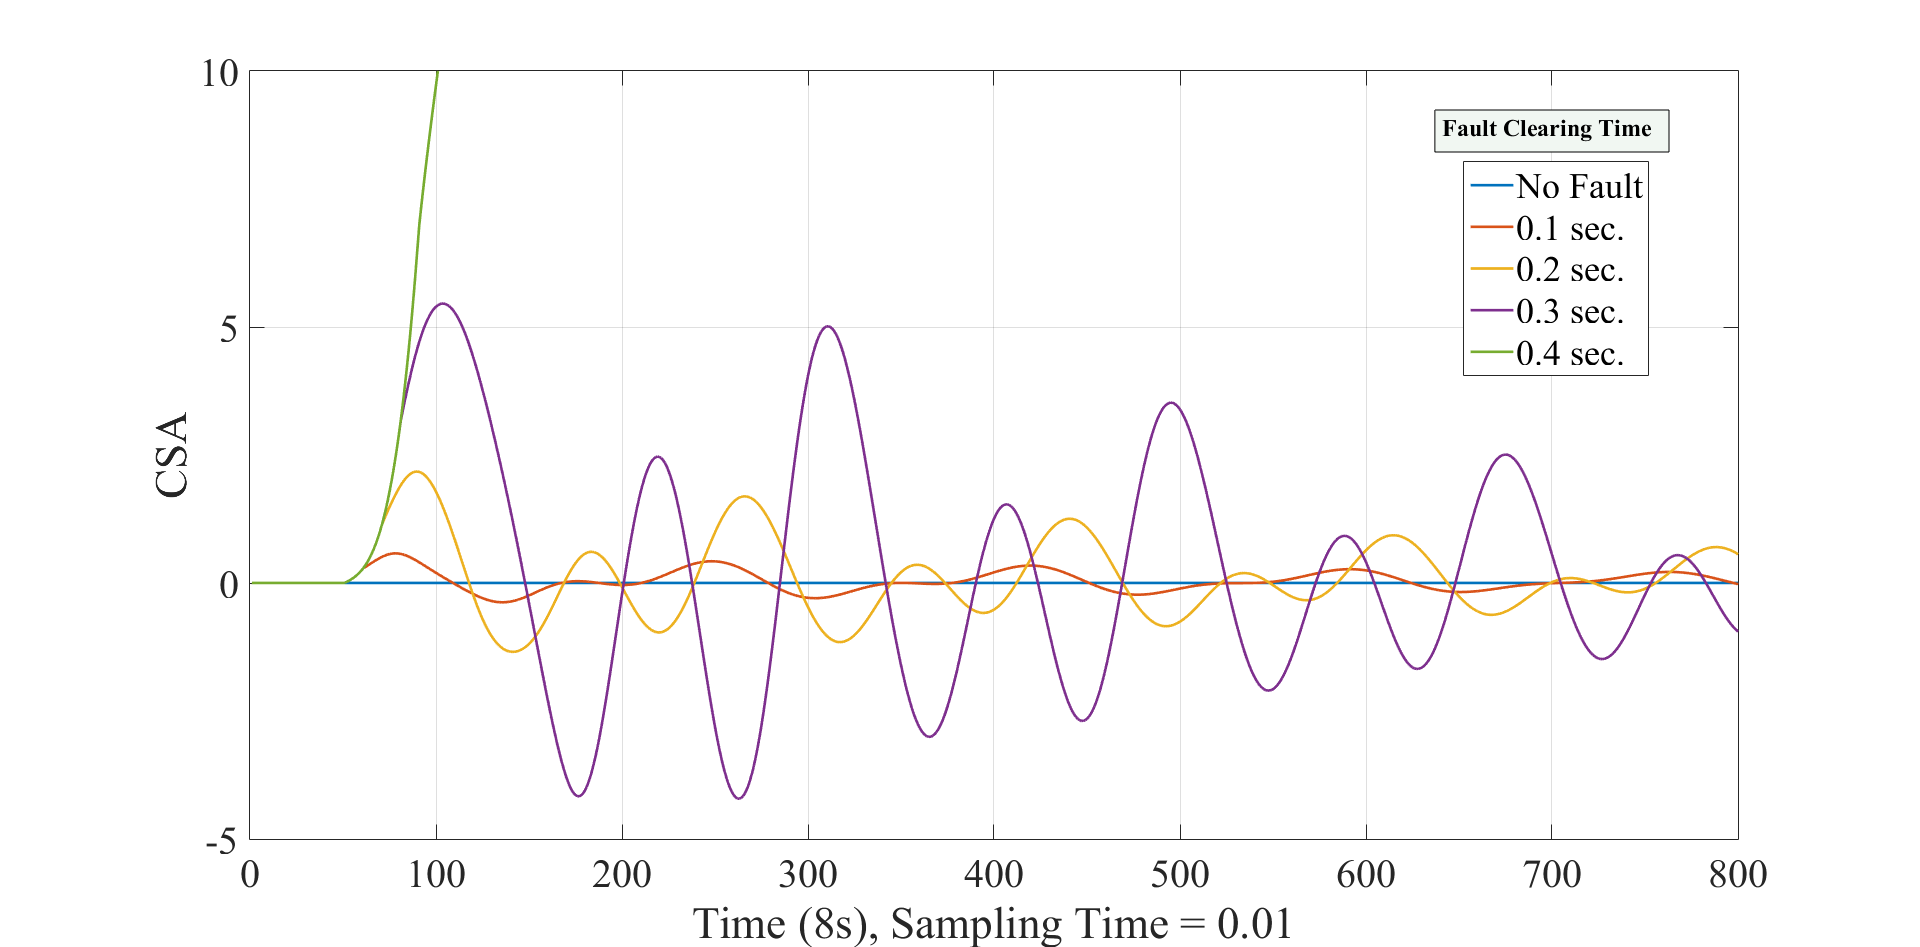
\includegraphics[width=\linewidth]{CSA}
  \caption{Contingency Severity Assessment (CSA)}
  \label{fig:I4}


\end{figure}

\begin{table}[H]
\renewcommand{\arraystretch}{1}
\caption{Contingency Analysis using Indicator based on Dot Products (CSA)}
\label{Table:I3}
\begin{center}
\begin{tabular}{|P{0.3\linewidth} | P{0.3\linewidth} | P{0.2\linewidth}|}
\hline
 \textbf{Fault Clearing Time} & \textbf{Performance Index} & \textbf{Remarks}  \\ \hline
 No Fault & 1.5902e-10  & Stable \\ \hline
 0.1 sec & 0.9557  & Stable \\ \hline
 0.2 sec & 3.5214  & Stable \\ \hline
 0.3 sec & 9.6711  & Stable \\ \hline
 0.4 sec & 2.4770e+03  & Unstable \\ \hline
 
\end{tabular}
\end{center}
\end{table}



\subsection{Results for Wide Area Severity Index (WASI)}
\label{Ind4}
\begin{figure}[H]
  \centering
  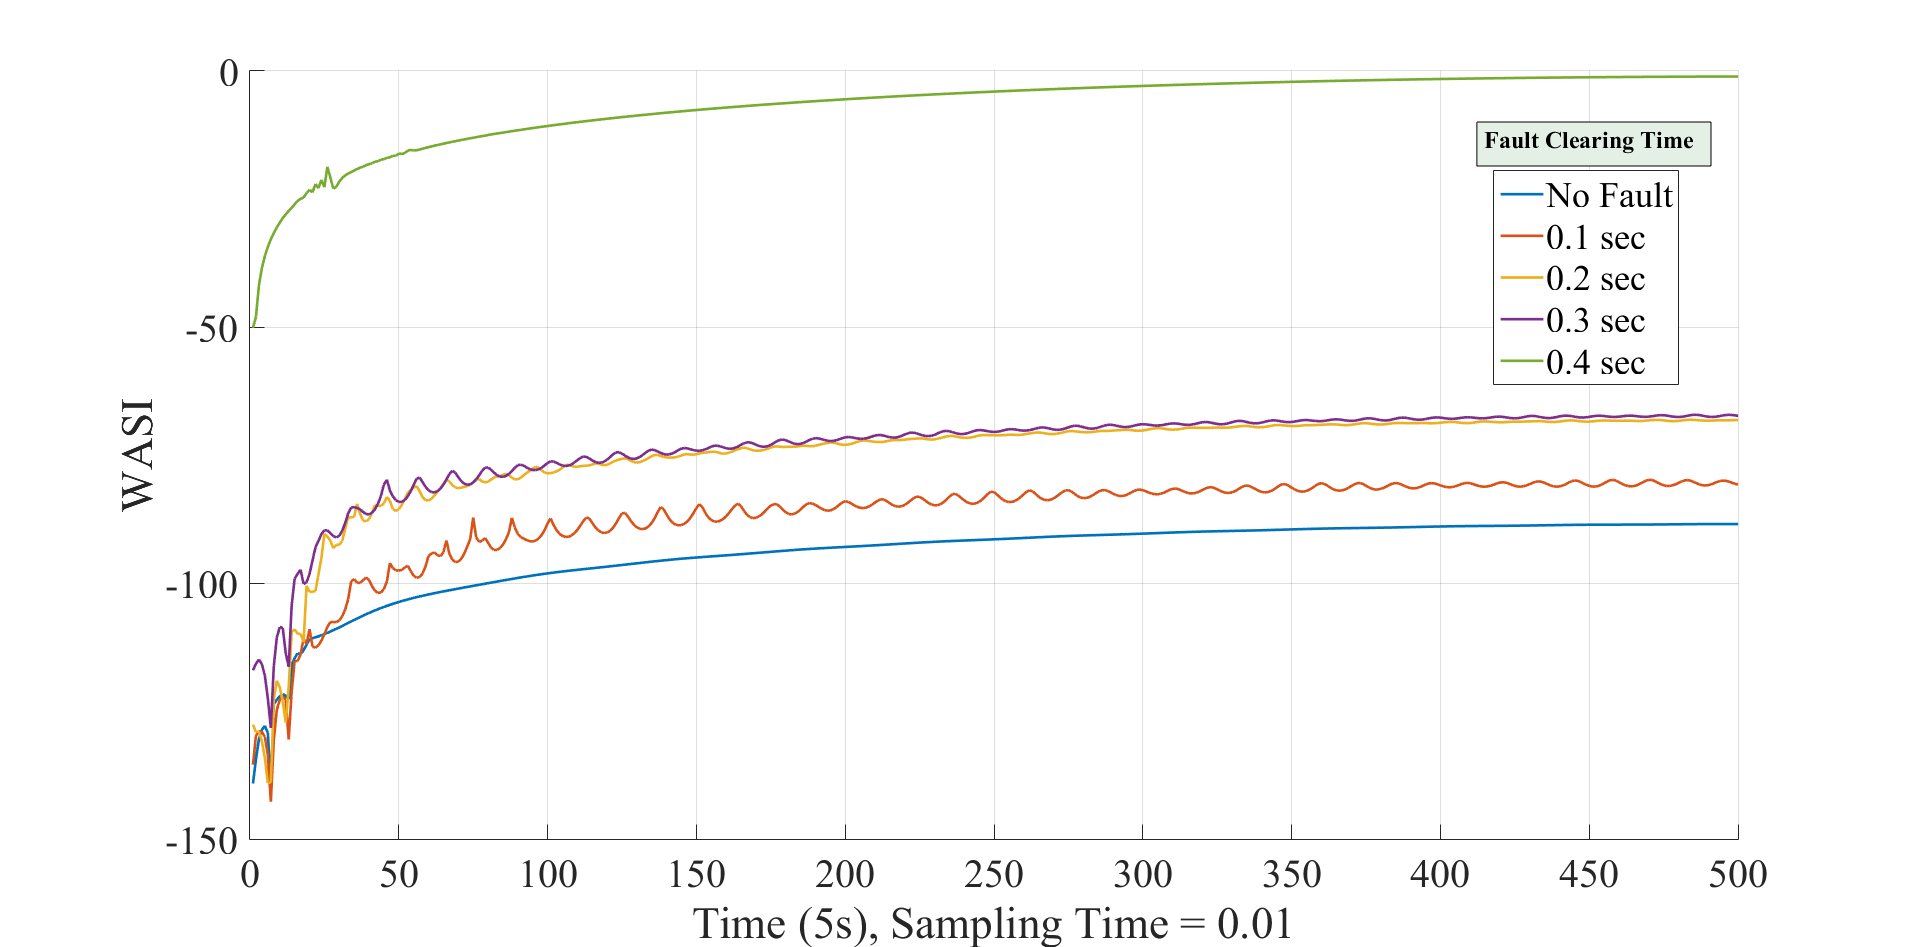
\includegraphics[width=\linewidth]{WASIcurve}
  \caption{Wide Area Severity Index (WASI)}
  \label{fig:I3}


\end{figure}

\begin{table}[H]
\renewcommand{\arraystretch}{1}
\caption{Contingency Analysis using Wide Area Severity Index (WASI)}
\label{Table:I4}
\begin{center}
\begin{tabular}{|P{0.3\linewidth} | P{0.3\linewidth} | P{0.2\linewidth}|}
\hline
 \textbf{Fault Clearing Time} & \textbf{Performance Index} & \textbf{Remarks}  \\ \hline
 No Fault & -88.4891  & Stable \\ \hline
 0.1 sec & -80.7781  & Stable \\ \hline
 0.2 sec & -68.1678  & Stable \\ \hline
 0.3 sec & -67.3590  & Stable \\ \hline
 0.4 sec & -1.0775  & Unstable \\ \hline
 
\end{tabular}
\end{center}
\end{table}


\subsection{Results for Inter-area Stability Prediction Index (ISPI)}
\label{Ind5}
\begin{table}[H]
\renewcommand{\arraystretch}{1}
\caption{Contingency Analysis using Inter-area Stability Prediction Index (ISPI)}
\label{Table:I5}
\begin{center}
\begin{tabular}{|P{0.3\linewidth} | P{0.3\linewidth} | P{0.2\linewidth}|}
\hline
 \textbf{Fault Clearing Time} & \textbf{ISPI} & \textbf{Remarks}  \\ \hline
 No Fault & 0.0000  & Stable \\ \hline
 0.1 sec & 3.1537  & Stable \\ \hline
 0.2 sec & 11.6207  & Stable \\ \hline
 0.3 sec & 31.9145  & Stable \\ \hline
 0.4 sec & 82.5676  & Unstable \\ \hline
 0.5 sec & 92.5350  & Unstable \\ \hline
 
\end{tabular}
\end{center}
\end{table}

\begin{figure}[H]
  \centering
  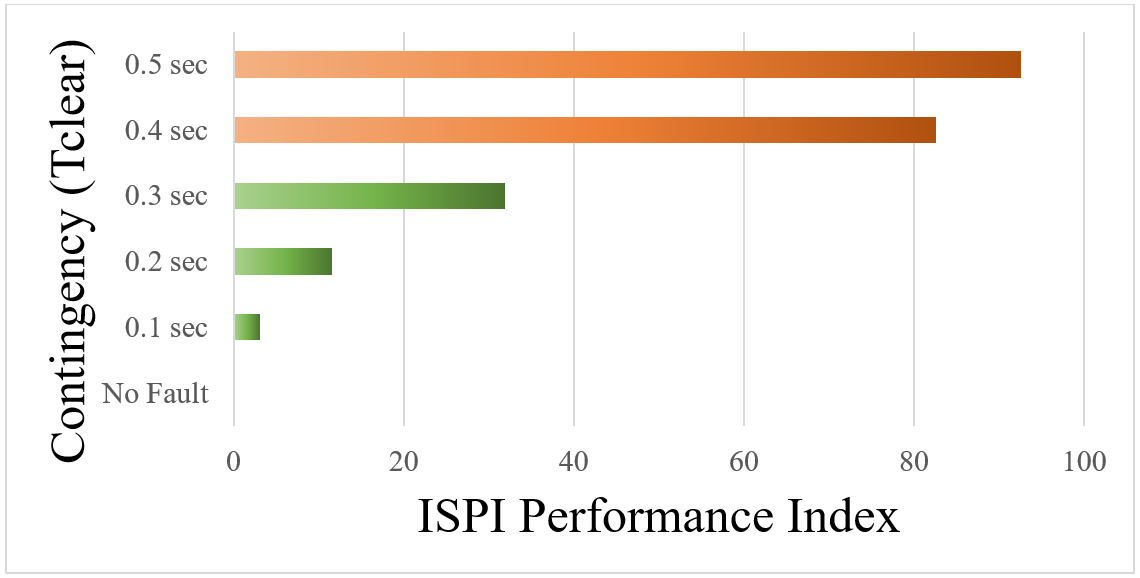
\includegraphics[width=\linewidth]{ISPI Bar graph}
  \caption{Inter-area Stability Prediction Index}
  \label{fig:I5}


\end{figure}

\section{Stability Analysis in Other Test Systems}
\label{R_Contingency}

\begin{table}[H]
\renewcommand{\arraystretch}{1}
\caption{Stability Analysis in Different Contingencies}
\label{Table:R_Contingency}
\begin{tabular}{|P{1.9 cm} | P{1.9 cm} | P{1.9 cm}|P{1.9 cm} | P{1.9 cm} | P{1.9 cm}| P{0.6 cm}|}
\hline
  
  \textbf{\textit{Fault Clearance Time}}  & \textbf{Coherency based Indicator} & \textbf{TEC based Indicator} & \textbf{CSA Indicator} & \textbf{WASI Indicator} & \textbf{ISPI Indicator} & \textbf{R*} \\\hline
 
    \bottomrule
    \bottomrule
    \multicolumn{7}{P{14 cm}}{\textit{\textbf{Contingency 1:} \textbf{145}-Bus, \textbf{50}-Machine System  \textbf{||}  Fault on Bus-\textbf{100}  \textbf{||}  Line Tripped between Bus-\textbf{100} and Bus-\textbf{103}}}\\\hline
    
    \textbf{0.1 sec} & 0.7925 & 1.1139 & 6.0352 & -132.6903 & 19.9160 & S\\\hline
    \textbf{0.2 sec} & 1.9300 & 2.3566 & 17.9379 & -81.9617 & 33.3588 & S\\\hline
    \textbf{0.3 sec} & 1.3248e+03 & 2.6497e+03 & 3.7071e+05 & -9.2605 & 100 & U\\\hline
    \textbf{0.4 sec} & 1.3913e+03 & 2.7826e+03 & 3.9845e+05 & -6.9247 & 100 & U\\\hline
     
     \bottomrule
    \multicolumn{7}{P{14 cm}}{\textit{\textbf{Contingency 2:} \textbf{10}-Bus, \textbf{4}-Machine System  \textbf{||}  Fault on Bus-\textbf{8}  \textbf{||}  Line Tripped between Bus-\textbf{7} and Bus-\textbf{8}}}\\\hline
    
    \textbf{0.1 sec} & 0.3341 & 0.6311 & 0.4248 & -78.2523 & 1.4020 & S\\\hline
    \textbf{0.2 sec} & 0.5372 & 0.8180 & 0.7497 & -77.2143 & 2.4740 & S\\\hline
    \textbf{0.3 sec} & 0.8436 & 1.1307 & 1.7686 & -75.2880 & 5.8365 & S\\\hline
    \textbf{0.4 sec} & 1.2719 & 1.2682 & 3.8308 & -63.7517 & 12.6416 & S\\\hline
    \textbf{0.5 sec} & 1.8062 & 2.1298 & 8.9612 & -62.0844 & 29.5719 & S\\\hline
    \textbf{0.6 sec} & 28.7068 & 46.7095 & 317.4158 & -4.7632 & 66.0481 & U\\\hline
    \textbf{0.7 sec} & 38.9884 & 66.7956 & 382.7585 & -1.3148 & 66.0580 & U\\\hline
    
    \bottomrule
    \multicolumn{7}{P{14 cm}}{\textit{\textbf{Contingency 3:} \textbf{145}-Bus, \textbf{50}-Machine System  \textbf{||}  Fault on Bus-\textbf{7}  \textbf{||}  Line Tripped between Bus-\textbf{7} and Bus-\textbf{8}}}\\\hline
    
    \textbf{0.01 sec} & 0.3215 & 0.1923 & 2.2805 & -240.8413
 & 7.5255 & S\\\hline
    \textbf{0.05 sec} & 1.6974 & 0.8372 & 20.5659 & -217.2081 & 33.4113 & S\\\hline
    \textbf{0.1 sec} & 78.1968 & 153.5396 & 6.6780e+03 & -2.7570 & 66.7798 & U\\\hline
    
\end{tabular}
\end{table}
\textbf{* R} - Remarks, \textbf{S} - Stable, \textbf{U} - Unstable

\section{Discussion}
For illustration of applicability of aforementioned catastrophic
indicators 4 contingencies are taken as example in previous sections. The first contingency discussed in section \ref{contingency1} is the IEEE 10 Bus 4 Machine System, in which a fault is applied on Bus 9 and the fault is eliminated by releasing the connection between Bus-9 and Bus-10 at different fault clearing periods. Results of Indicators are analysed through curves (refer Fig. \ref{fig:I1} to Fig. \ref{fig:I4}) as well as in tabular form (refer Fig. \ref{Table:I1} to Fig. \ref{Table:I5}). For Indicator 1 i.e. Indicator based on Coherency results are provided in section \ref{Ind1} shows 5 figures for each Fault Clearing Time including No fault. The data are observed clearly that for no fault and 0.1 sec, 0.2 sec and 0,3 sec the curves of generator speed are deviating gradually but in 0.4 sec there is larger deviation and its peak is at 66.9471 p.u. i.e Performance Index for 1st Indicator where as PI (Performance index) is very much small in other four Tclear times. Similar situation in Indicator 2 i.e. Indicator based on Transient Energy Conversion (refer section \ref{Ind2}), Performance Index for 0.4 sec Tclear is 133.8941, where as for other four cases it is less than 3 p.u. The difference between Kinetic and potential energy is much higher for Tclear =0.4 sec. So, it is obvious that system is not in stable state. In section \ref{Ind3} third Indicator i.e. Indicator based on Dot Products (CSA)
results are defined and its in single curve because the PI is produced in single curve (refer fig. \ref{fig:I3}). For each Tclear time one curve of specific color is drawn from algorithm for the taken contingency and the reference color data can be guided from legend provided on curve. From the curve can also one can distinguish between stable and unstable cases. The deviation here is also refers the Performance Index. Its tabular data shows the deviation upto Tclear 0.3 sec starting from No fault is 9.6711 and on 0.4 sec Tclear it reaches to 2.4770e+03. These 3 indicators posses same pattern and all are clearly indicating the system condition. The large gap in numbers and in curves itself is the proof of Indicator working. Its not always not possible to plot each and every system in plots because of high power ratings, so, indicator 4 i.e. Wide Area Severity Index (WASI) (results are discussed in section \ref{Ind4}). As it is in logarithmic form so higher values are compressed to minimum value possible so it is each to observe through machines. The PI of WASI is different from discussed above 3 methods and it is observed that result occurs in -y axis. But similar to them, here also there is large difference in values between stable and unstable condition. Fifth Indicator i.e. Inter-area Stability Prediction Index (ISPI) (results are discussed in section \ref{Ind5}) produces results in percentage and it is previously defined in section \ref{ISPI_Intro} that for how much percentage the system is stable and for what it is unstable. Now the data are produced in both tabular and graphical form manually collected from algorithm and observed that for Tclear 0.3 sec and below the PI is below 33\% and for Tclear = 0.4 sec the PI is 82.5676\%, which is in alarming state. So, both the data(Graphical as well as Tabular) shows for Tclear = 0.1 sec, 0.2 sec, 0.3 sec the system behaves stable performance after fault, but for Tclear = 0.4 sec system moves to unstable state. So, the Threshold Tclear lies between 0.3 sec and 0.4 sec and it is found to be 0.318 sec when it is executed manually. Analysis of Indicator states that all the Indicator has different Threshold values (not Threshold Tclear). Similarly in section \ref{R_Contingency} other three contingencies are performed for Indicator Analysis. The Indicator performances are described in Table \ref{Table:R_Contingency}, the results (behaviour of the system, i.e. Stable or Unstable) for all the aforementioned catastrophic indicators are same for a particular value of Tclear.
